\newcommand{\numfoil}{\textsf{numfoil}}
\newcommand{\xfoil}{\textsf{XFOIL}\ }
\chapter{Problem Description}
To get a preliminary estimation of an airfoil's performance, numerical methods
can be used which represent the airfoil as a series of flat, zero-thickness,
panels. Various kinds of singularities can then be placed on those panels to
manipulated the airflow around them to resemble the flow behavior around the
actual airfoil.\\

In this part of the report, two separate methods will be discussed.
The first method ignores the airfoil's thickness and instead reduces it to only
a set of $n$ panels located on the camber line. A lumped vortex element is then
placed at some location on each panel, as well as a collocation point. At each
collocation point, the influence of all these vortex elements will be evaluated.
From this, values like $C_l$, $C_m$ and $C_p$ can be estimated. Using this
method the effect of camber on the airfoil can be quickly evaluated.\\

To also evaluate the effect of thickness, the second method instead places $n$
panels along the airfoil's surface. This time a linear distribution of vortex
elements are placed in the panels. Both methods are based on the Kutta
condition, meaning this condition is intrinsically satisfied. Both methods have
the same general structure, which can be seen in \autoref{fig:activity}. The
steps are discussed in more detail for each of the two methods in the following
sections.

\chapter{Implementation}
For this assignment, the goal was to both learn more about potential flow
theory while simultaneously creating a high-performance Python package making
use of JIT compilation for parallelization. Doing so enabled use of modern
hardware while representing multiple airfoil discretizations ranging from thin
airfoils to also thick paneling methods. The object-oriented paradigm, along
with SOLID architecting principles was applied to create abstractions that
could be specialized per type of potential flow solver. Doing so allowed
minimal code duplication between each panel method, and resulted in the
\numfoil\footnote{\url{https://github.com/skilkis/numfoil}} package which is
publically available. Open sourcing the package is done in the spirit of
helping future students understand the theory given within textbooks from a
clean-code perspective, which was not previously possible due to the scripting
implementations within those textbooks being void of information as a result of
obscure variable names.\\

\begin{wrapfigure}{R}[2em]{0.55\textwidth}
    \vspace{-2em}
    \begin{center}
      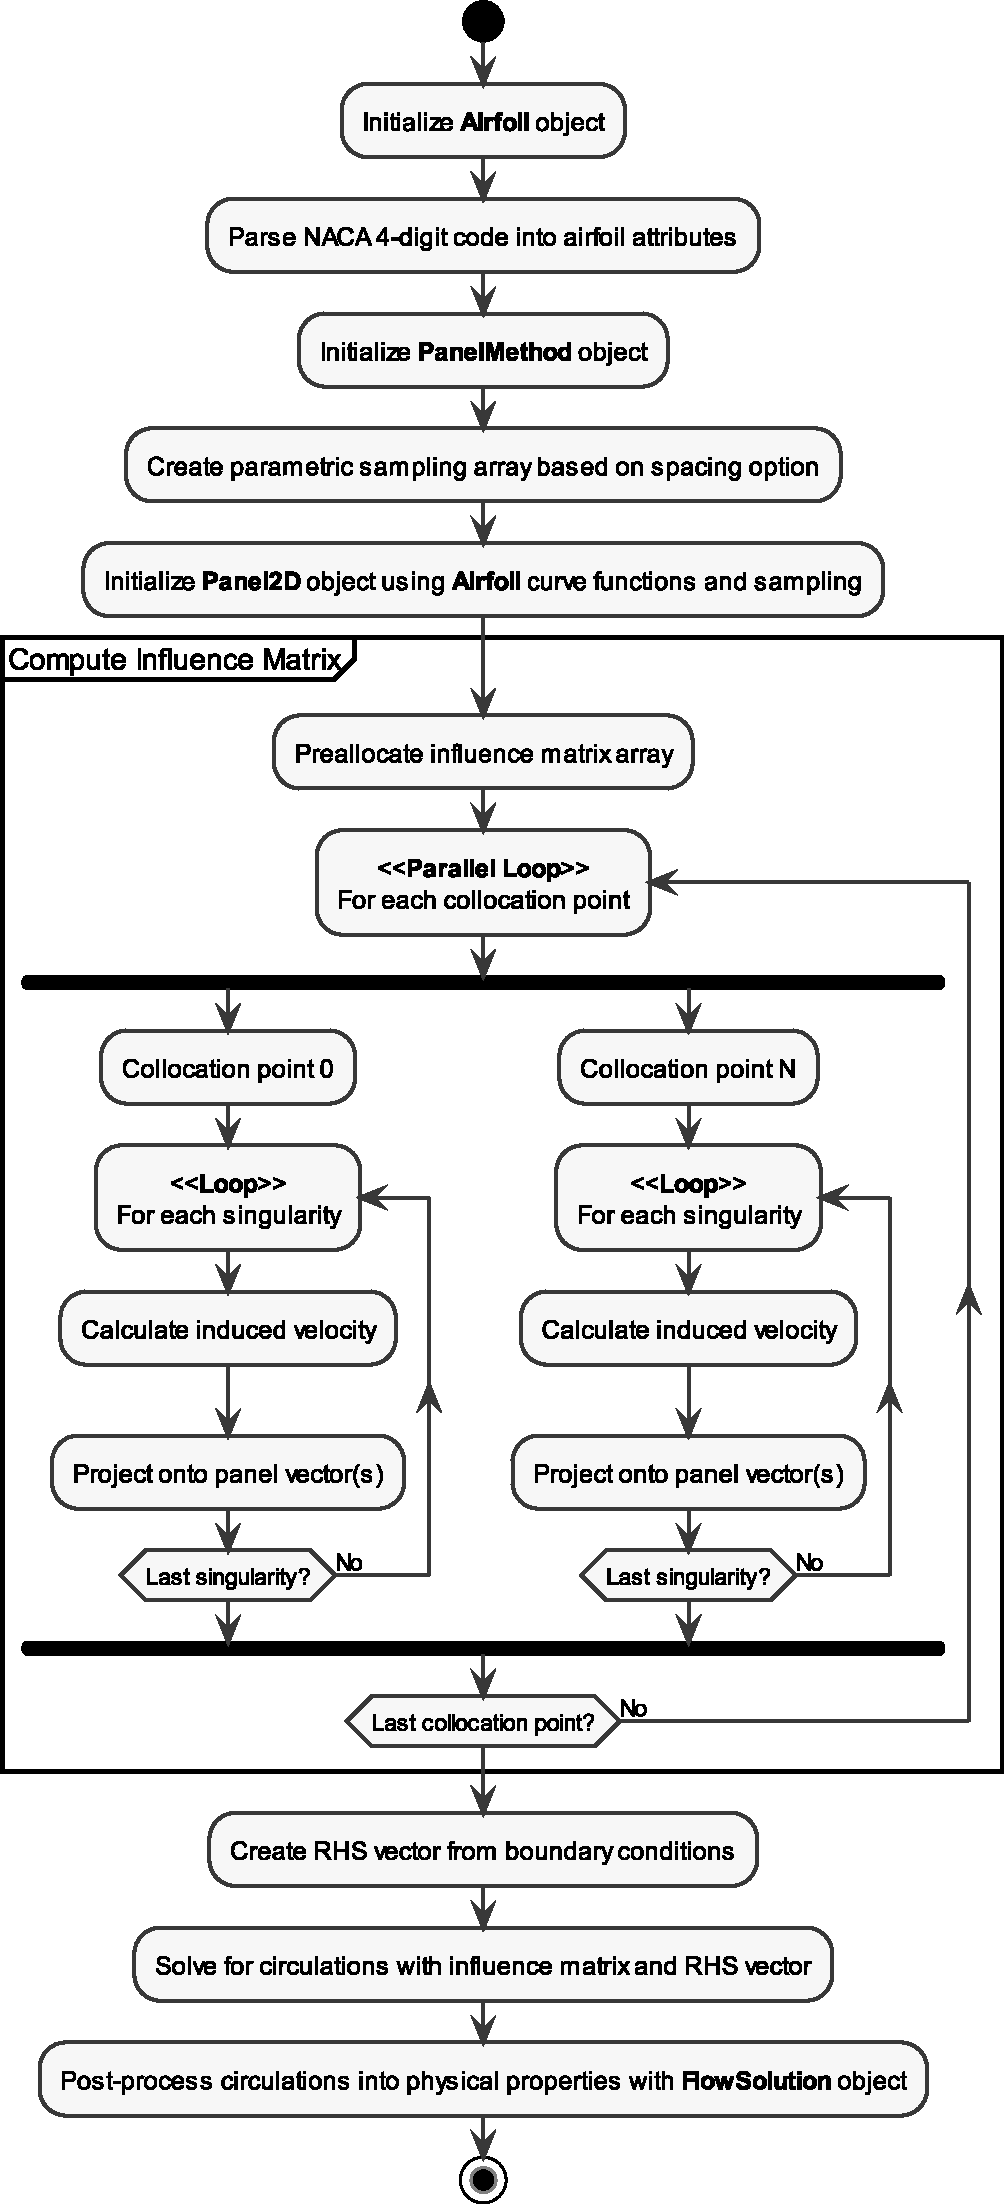
\includegraphics[width=0.40\textwidth]{static/activity_diagram.pdf}
    \end{center}
    \caption{UML Activity Diagram of \numfoil}
    \label{fig:activity}
\end{wrapfigure}

In the development process of \numfoil, multiple panel methods were
investigated to establish abstractions that were universal. From this
investigation, the resulting abstraction is to understand how 2D airfoil panel
methods discretize a contour, placing singularities at pre-determined
locations, and measure their influence at other pre-determined locations called
collocation points. The combined influences of all vortices can then be used
along with boundary conditions that enforce flow penetration and tangency
constraints to solve a system of linear equations. The general flow of all of
these approaches is then, a) discretize the geometry, b) place singularity and
collocation points to determine the influence these signularities will have, c)
set boundary conditions on the system, and finally d) solve the resulting
system of linear equations to obtain the circulations which can then be post
processed into desired quantities of lift and pressure coefficient.\\

These steps are then treated as responsibilities and split-up into different
modules of the \numfoil package. To explain the flow of the code better, a UML
activity diagram has been created, \cref{fig:activity}. In this diagram, one
can see that first the \textsf{Airfoil} class is responsible for defining the
geometry of the airfoil at any distance x along the chord-line. \\

The user can then pass in the \textsf{Airfoil} object to a \textsf{PanelMethod}
class which then is responsible for querying the airfoil at various locations
to produce a paneled geometry of the airfoil. This geometry is then represented
by a \textsf{Panel2D} object which has additioanl data such as the normal and
tangent vectors of each panel. Once the panelling is completed, the geometry is
used to construct an influence matrix. In this step the influence of all
singularities on a particular panel, is independent of other panels due to the
initial assumption that the circulation strength is one and can therefore be
massively parallelized. This is depicted in \cref{fig:activity} by the
Collocation Point 0 and Collocation Point N being solved in parallel.\\

Once the influence matrix is constructed, depending on the panel method used,
the flow velocity is projected either on the normal or tangent vector of each
panel. This allows for creating a Right Hand Side (RHS) vector which then
presents a system of linear equations. Through matrix inversion, the unknown
circulation strengths can then be solved for. Finally, the circulation
strengths can then be processed into the desired flow quantities using the
\textsf{FlowSolution} class.

\section{Geometry Definition}
Before we can begin the analysis, the functions describing the desired
airfoil's camber line, and upper and lower surface should be created. Airfoils
are defined using the NACA 4-digit code. \autoref{eq:camber} is used to obtain
the camber line function.

\begin{equation}
\label{eq:camber}
    y_{c}=\left\{
        \begin{array}{ll}
            \frac{m}{p^{2}}\left(2 p\left(\frac{x}{c}\right)-\left(\frac{x}{c}\right)^{2}\right),
            & 0 \leq x \leq p c \\
            \frac{m}{(1-p)^{2}}\left((1-2 p)+2 p\left(\frac{x}{c}\right)-\left(\frac{x}{c}\right)^{2}\right),
            & p c \leq x \leq c
        \end{array}\right.
\end{equation}
\medskip

Here $m$ is the maximum camber and $P$ is the location of the maximum camber, or
the first and second digit of the 4-digit NACA code divided by ten respectively.
Subsequently, to find the coordinates of the upper and lower airfoil
surface, the thickness is applied perpendicular to the camber line using
\autoref{eq:coor_u} and \autoref{eq:coor_l} respectively, where $\theta =
\arctan\left( \frac{y_c}{dx}\right)$.

\begin{equation}
\label{eq:coor_u}
    \left(\begin{array}{l} x_U, \: y_U\end{array}\right) =
    \left(\begin{array}{l} x-y_t \sin \theta, \: y_c+y_t\cos \theta\end{array}\right)
\end{equation}
\begin{equation}
\label{eq:coor_l}
    \left(\begin{array}{l} x_L, \:  y_L\end{array}\right) =
    \left(\begin{array}{l} x+y_t \sin \theta, \: y_c-y_ t \cos \theta\end{array}\right)
\end{equation}

\chapter{Panel Methods}  % TODO Decide if this should be a section?
Two different methods well be implemented to perform basic airfoil analysis.
First, the airfoil is represented by its camberline only, and thus has a
thickness of zero. The results of this method will be compared with the second
method, which discretizes the airfoil by placing panels on the outer surface
instead. Hence, this second method does take airfoil thickness into account.

\section{Lumped Vortex Method}
\label{sec:thin}
The first method, described by \citeauthor{katz_plotkin}\cite{katz_plotkin}, analyzes an airfoil
looking only at the airfoil's camber line. This discretization is visualized in
\autoref{fig:discr_thin}, where $n=7$ panels are placed on the camber line starting at
the leading edge. These panels are created by adding $n+1$ nodes on the camber
line, the coordinates for which are obtained using the camber line function from
\autoref{eq:camber}. Lumped vortex elements and collocation points are placed at
25\% and 75\% of each panel's length. This way the airfoil is represented as a
set of zero-thickness vortex sheets.
% Note that linear node spacing is used in
% \autoref{fig:discr_thin}. For the implementation, however, cosine spacing is used to
increase accuracy of the results at the leading and trailing edge.


\begin{figure}[H]
\centering
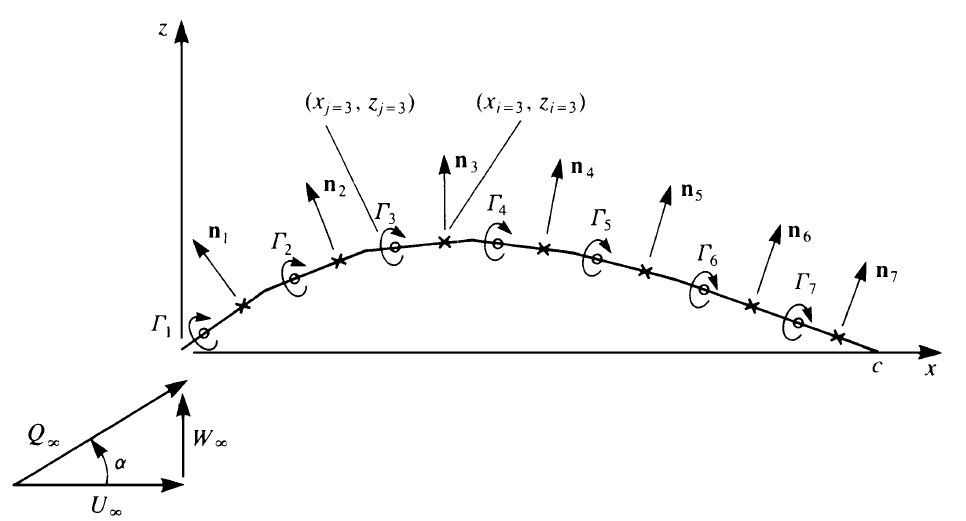
\includegraphics[width=.8\textwidth]{static/disc_camber.png}
\caption{Discretization of the airfoil camber line using $n=7$ panels \cite{katz_plotkin}}
\label{fig:discr_thin}
\end{figure}

\subsection{Equations}
The normal velocity, which consists of the free-stream velocity and the
self-induced velocity, must be zero at each point along the camber line. This
way the camber line is set to be a streamline of the free-stream. This
boundary condition is described by \autoref{eq:thin_cond}. Here,
$\vec{\bf{n}}_i$ is the normal vector of the $i-$th panel given by
\autoref{eq:normal}, and $\alpha_i$ is the angle w.r.t. the x-axis of the $i-$th
panel.

\begin{equation}
\label{eq:thin_cond}
    \left( u_i, \: w_i \right) \cdot \vec{\bf{n}}_i + \left( U_\infty,
    \: W_\infty \right) \cdot  \vec{\bf{n}}_i = 0
\end{equation}
\begin{equation}
\label{eq:normal}
    \vec{\bf{n}}_i = \left( \sin \alpha_i, \: \cos \alpha_i \right)
\end{equation}

Next, if $\left( x_i, \: y_i \right)$ is the location of the $i-$th panel
collocation point, and $\left( x_j, \: y_j \right)$ is the location of the
$j-$th vortex element, the velocity induced at each collocation point due to
the presence of the $n$ vortices, with strength $\Gamma_j$, is found using
\autoref{eq:v_ind_thin}. Note that an error exists within the textbook, as to
represent a correct induced velocity due to the $j-$th vortex element which are
clock-wise rotating, a clock-wise affine transform must be used. Originally, a
counter-clockwise affine transform is provided in \cite{katz_plotkin}.
\medskip

\begin{equation}
\label{eq:v_ind_thin}
    \left(\begin{array}{l}
    u_i \\ w_i
    \end{array}\right)
    =
    \sum_{j=1}^{n} \:
    \left[ \frac{\Gamma_{j}}{2 \pi r_{i,j}^{2}}
    \left(\begin{array}{cc}
    0 & -1 \\ 1 & 0
    \end{array}\right)
    \left(\begin{array}{l}
    x_i-x_{j} \\ z_i-z_{j}
    \end{array}\right) \right], \; \; \; \; \; \forall \; i \in \{1,...,n\}
\end{equation}
\begin{equation}r_{j}^{2}=\left(x_i-x_j\right)^{2}+\left(z_i-z_j\right)^{2}\end{equation}
\medskip

Naturally, if $i=j$, the respective collocation point and vortex are located
on the same panel. The vorticities, $\Gamma_j$, are the unknown which will be solved for.
Combining \autoref{eq:v_ind_thin} with \autoref{eq:thin_cond}, and moving the free-stream
velocity from \autoref{eq:thin_cond} to the right hand side of the equation,  yields a
system of $n$ equations which can be solved algebraically to find the vorticity of each vortex element.
Once the vorticity $\Gamma_j$ is known for each vortex element, the change in lift and
pressure are obtained using \autoref{eq:thin_lift} and \autoref{eq:thin_press} respectively \cite{katz_plotkin}.
 $s_i$ is the length of the $i-$th panel.

\begin{minipage}{.5\linewidth}
\begin{equation}
\label{eq:thin_lift}
\Delta L_i = \rho v_\infty \Gamma_{j=i}
\end{equation}
\end{minipage}%
\begin{minipage}{.5\linewidth}
\begin{equation}
\label{eq:thin_press}
\Delta P_i = \rho v_\infty \frac{\Gamma_{j=i}}{s_i}
\end{equation}
\end{minipage}%

\subsection{Verification}
The results of the lumped vortex panel method are verified by comparing them to
analytical data from an equation by \citeauthor{katz_plotkin} for an elliptical
camberline. The camberline shape is given by \cref{eq:ellipticcamber}, and the
respective pressure differential is given by \cref{eq:cpell}. The pressure
differential distributions are plotted for two values of $\varepsilon$ and $\alpha$
in \cref{fig:thin_verif}. The plots labeled with the angle of attack are the
ones obtained with the created tool (\numfoil). The plots labeled `exact solution' were
created using \cref{eq:cpell}. Finally, the pressure differential was calculated
by subtracting the pressure distributions of the upper and lower surface of an
airfoil as obtained from \xfoil. In order to get results for a near-flat plate, elliptical
camberline, the airfoil in \xfoil was set to a NACAX501 airfoil. Here the X takes
on the value of camber corresponding to $X = 100\varepsilon$.
The value of angle of attack $\alpha$ is capped at \SI{7}{\degree}, as \xfoil does
not converge to a pressure distribution solution for larger values.

\begin{equation}
  \label{eq:ellipticcamber}
  \eta(x) = 4 \varepsilon \frac{x}{c} \left[ 1 - \frac{x}{c} \right]
\end{equation}
\begin{equation}
  \label{eq:cpell}
  \Delta C_p = 4 \sqrt{\frac{c-x}{x}}\alpha + 32 \frac{\varepsilon}{c}\sqrt{\frac{x}{c}\left( 1- \frac{x}{c}\right)}
\end{equation}
\medskip

\begin{figure}[h]
  \centering
  \begin{subfigure}{.5\textwidth}
    \centering
    \captionsetup{width=.8\linewidth}
    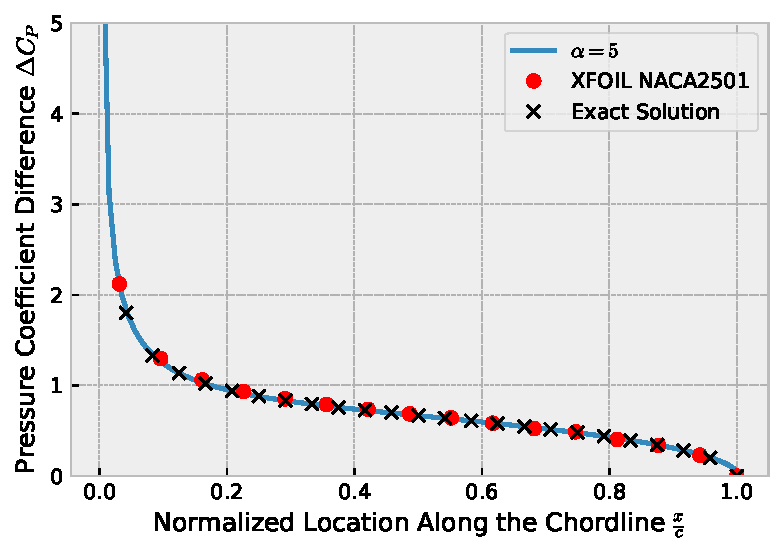
\includegraphics[width=.9\linewidth]{static/thin_airfoil_verification_a5.pdf}
    \caption{\centering Pressure differential distribution for $\epsilon = 0.02$ at $\alpha = 5^{\circ}$}
    \label{fig:thin_verif1}
  \end{subfigure}%
  \begin{subfigure}{.5\textwidth}
    \centering
    \captionsetup{width=.8\linewidth}
    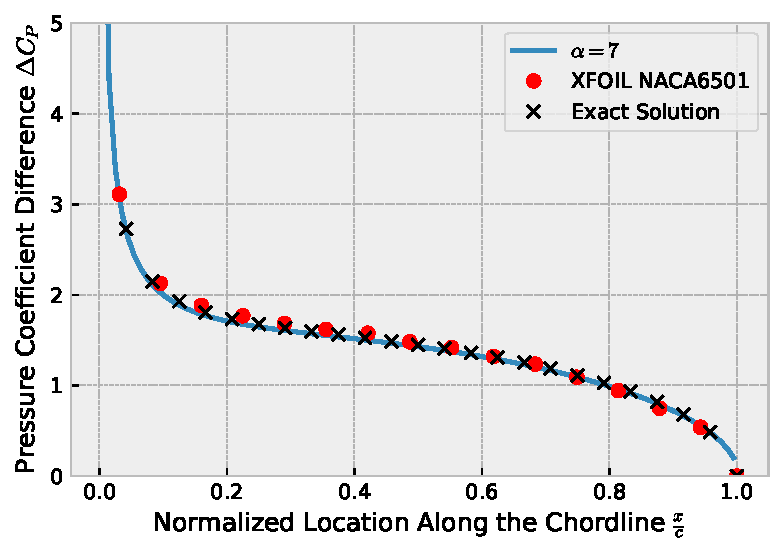
\includegraphics[width=.9\linewidth]{static/thin_airfoil_verification_a7.pdf}
    \caption{\centering Pressure differential distribution for $\epsilon = 0.06$ at $\alpha = 7^{\circ}$}
    \label{fig:thin_verif2}
  \end{subfigure}
  \caption{\centering Verification of lumped vortex method results by comparing with the analytical solution for elliptical camber \cite{katz_plotkin}}
  \label{fig:thin_verif}
\end{figure}

The lift coefficients are verified by comparing once more to data obtained from
\xfoil. This time, a simple flat plate is approximated by the NACA0001 airfoil,
and a camberline of a NACA24XX airfoil by setting the thickness as low as
possible, i.e. NACA2401. Resulting lift coefficients for a sequence of angle of
attack values are listed in \cref{tab:cl_thin}. For the near-flat plate, the
error does not exceed $1.4\%$, while for the camberline, the error reaches
values up to $4.75\%$ at higher angles of attack.
% These results should be taken
% with a grain of salt, as flat plates have zero-radius leading edges which cause
% suction peaks of possible infinite magnitude, which neither method might account
% for correctly.

\begin{table}[]
	\centering
	\caption{Estimated values of $C_l$ for a range of angles of attack from \xfoil and NumFoil, as well as the relative error, for NACA0001 and NACA2401.}
	\label{tab:cl_thin}
    \begin{tabularx}{\textwidth}{C  C C C | C C C} %'L' for Left Aligned, 'C' for Centered, 'R' for Right Aligned
    \toprule\
    \hfill & \multicolumn{3}{c}{$C_l$ NACA0001} & \multicolumn{3}{c}{$C_l$ NACA2401} \\ \toprule
    {$\alpha \:[\deg]$} & {$NumFoil$} & {$\xfoil$} & {$\epsilon$} & {$NumFoil$} & {$\xfoil$} & {$\epsilon$} \\ \toprule
    0   & 0        & 0      & 0         & 0.2266 & 0.2302  & -0.0155    \\ \hdashline
    3   & 0.3288   & 0.3335 & -0.0139   & 0.5552 & 0.5599  & -0.0084    \\ \hdashline
    5   & 0.5476   & 0.5550 & -0.0133   & 0.7735 & 0.7729  & +0.0007    \\ \hdashline
    8   & 0.8744   & 0.8843 & -0.0111   & 1.0990 & 1.0810  & +0.0167    \\ \hdashline%\midrule
    10  & 1.0911   & 1.1010 & -0.0090   & 1.3144 & 1.2781  & +0.0284    \\ \hdashline
    13  & 1.4134  & 1.4204 & -0.0049   & 1.6345 & 1.5604  & +0.0475     \\ \bottomrule
    \end{tabularx}
\end{table}

% ###########################################################################################
% ###########################################################################################

\section{Linear Vortex Model}
\label{sec:thick}
The second method, described by %\citeauthor{katz_plotkin}\cite{katz_plotkin},
\citeauthor{kuethe_chow_1998}\cite{kuethe_chow_1998}, places vortex elements
with linearly increasing strength in the center of panels on the airfoils
surface. The airfoil is discretized by placing $n$ nodes on the airfoil starting
at the trailing edge, over the lower airfoil surface to the leading edge and
back to the trailing edge over the upper surface. Each node presents a panel
edge, so there are $n-1$ panels. The same naming scheme as used in
\autoref{sec:thin} applies here too.

\subsection{Equations}
\label{ssec:eq_thick}
The boundary condition states that the normal velocity on the panels
must be zero, as described by \autoref{eq:thick_cond}\cite{kuethe_chow_1998}.
The Kutta-condition, shown in \autoref{eq:kutta}, is
added to ensure smooth flow transition to freestream at the trailing edge. This
results in one extra collocation point at the trailing edge, meaning that while
there are only $n-1$ panels, there are $n$ collocation points, the $n$-th one
representing the Kutta-condition.
\smallskip

\begin{minipage}{.5\linewidth}
\begin{equation}
  \label{eq:thick_cond}
  \frac{\partial}{\partial n_{i}} \phi\left(x_{i}, y_{i}\right)=0
  \end{equation}
\end{minipage}
% \begin{equation}
% \label{eq:thick_cond}
%     \left( U_\infty + u_i, \: W_\infty + w_i \right) \cdot \left( \cos \alpha_i,
%     \: -\sin \alpha_i \right) = 0
% \end{equation}
\begin{minipage}{.5\linewidth}
\begin{equation}
  \label{eq:kutta}
      \gamma_1 + \gamma_{n} = 0
\end{equation}
\end{minipage}
\smallskip

The velocity potential, $\phi$, in a collocation point at $(x_i,\: y_i)$ due
to $n-1$ vortices located at $(x_j, \: y_j)$ is obtained using
\autoref{eq:phi_thick}.
% When capital letters are used, $(X_j, \: Y_j)$ represent the panel's leading edge
% node, and $(X_{j+1}, \: Y_{j+1})$ refer to the panel's trailing edge node.
% Substituting \autoref{eq:phi_thick} in \autoref{eq:thick_cond} and applying it
% to every collocation point present will yield a system of $n$ equations which
% can be solved for the vorticities $\gamma_j$.

\begin{equation}
  \label{eq:phi_thick}
    \phi\left(x_{i}, y_{i}\right)=V_{\infty}\left(x_{i} \cos \alpha+y_{i} \sin \alpha\right)-\sum_{j=1}^{n-1} \int_{j} \frac{\gamma\left(s_{j}\right)}{2 \pi} \tan ^{-1}\left(\frac{y_{i}-y_{j}}{x_{i}-x_{j}}\right) d s_{j}
  \end{equation}
  \begin{equation}
    \gamma\left(s_{j}\right)=\gamma_{j}+\left(\gamma_{j+1}-\gamma_{j}\right) \frac{s_{j}}{S_{j}}
    \end{equation}
% \begin{equation}
% \label{eq:v_ind_thick}
%     \left(\begin{array}{l}
%     u_{p_i} \\ w_{p_i}
%     \end{array}\right)
%     =
%     \sum_{j=1}^{n} \:
%     \left(\begin{array}{c}
%     \frac{\gamma_j}{2\pi}\left[ \tan^{-1} \left(
%         \frac{z_i - z_{j+1}}{x_i - x_{j+1}}\right)
%          - \tan^{-1} \left( \frac{z_i - z_j}{x_i - x_j}\right) \right] \\[1em]
%     -\frac{\gamma_j}{4\pi} \ln \left[ \frac{\left( x_i - x_j \right)^2 +
%     \left( z_i - z_j \right)^2}{\left( x_i - x_{j+1}\right)^2 +
%     \left( z_i - z_{j+1} \right)^2 }  \right]
%     \end{array}\right), \; \; \; \; \; \forall \; i \in \{1,...,n\}
% \end{equation}
\medskip

% Once that the results of \autoref{eq:v_ind_thick} are in the local panel
% coordinate system and must be transformed back to the global one. Adding
% \autoref{eq:kutta} to the system of equations obtained from
% \autoref{eq:v_ind_thick}, will result in n+1 equations.
% \citeauthor{katz_plotkin}\cite{katz_plotkin} deals with this by replacing an
% arbitrary equation from the system with the Kutta condition, while
% \citeauthor{kuethe_chow_1998}\cite{kuethe_chow_1998} adds an equation, where the
% Kutta condition is altered as shown in \autoref{eq:kutta2}. Either way results
% in again an equal amount of equations and unknowns.
% \begin{equation}
%   \label{eq:kutta2}
%       \gamma_1 + \gamma_{n+1} = 0
% \end{equation}

Finally, \cref{eq:vind_thick} can be used to determine the induced velocity on a
panel due to all vortices present on the surface panels. For the details of this
linear vortex method and a simplified way to implement it by splitting up and
replacing large and complex equations with multiple coefficients
\citeauthor{kuethe_chow_1998}\cite{kuethe_chow_1998}
.
\begin{equation}
  \label{eq:vind_thick}
  V_{i}=\cos \left(\theta_{i}-\alpha\right)+\sum_{j=1}^{n} A_{i j} \gamma_{j}^{\prime}
\end{equation}

Once the vorticity $\gamma_j$ is known for each vortex element, the total lift
force is obtained using \autoref{eq:thick_lift}, where $\vec{\bf{L}}$ is the
lift direction obtained by rotating the free stream vector by \SI{90}{\degree},
and pressure coefficients are given by \autoref{eq:thick_press}.
\smallskip

\begin{minipage}{.5\linewidth}
\begin{equation}
\label{eq:thick_lift}
C_l = \sum_{i=1}^{n} C_{p_i} s_i \vec{\bf{n}}_i \cdot \vec{\bf{L}}
\end{equation}
\end{minipage}
\begin{minipage}{.5\linewidth}
\begin{equation}
\label{eq:thick_press}
C_{p_i} = 1 - v_i^2
\end{equation}
\end{minipage}

\subsection{Verification}
The linear vortex method with paneled airfoil surface is validated with data
obtained from \xfoil\cite{xfoil}. The pressure distribution found for two
different airfoils is shown in \autoref{fig:thick_verif}.
\autoref{fig:thick_verif1}  shows the results for
the NACA0015 at 5 degrees angle of attack, while \autoref{fig:thick_verif2} plots results for
the NACA2422 at 10 degrees angle of attack. Both have the respective results
obtained from \xfoil plotted on top of the results obtained with \numfoil. It can be seen
that the results coincide almost perfectly, with only negligible differences
observable at the suction peak on the upper surface leading edge.

\begin{figure}[h]
    \centering
    \begin{subfigure}{.5\textwidth}
      \centering
      \captionsetup{width=.8\linewidth}
      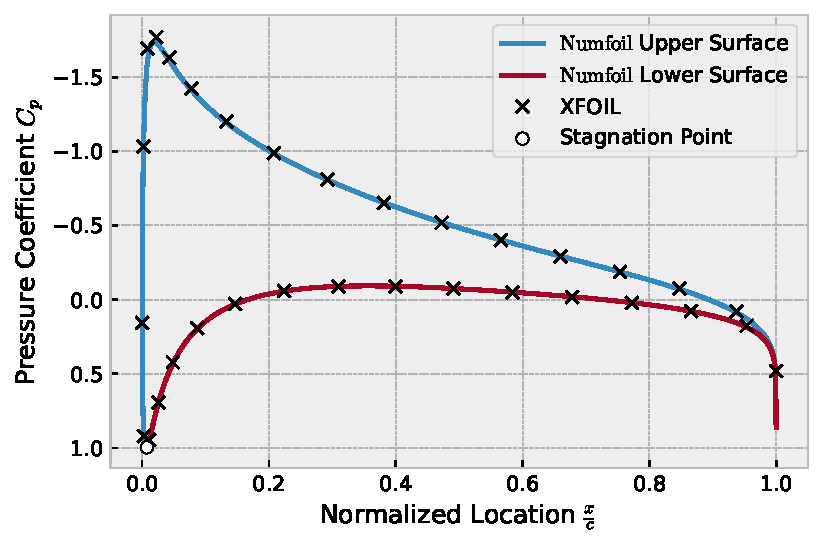
\includegraphics[width=.9\linewidth]{static/thick_verif_naca0015_alpha5.pdf}
      \caption{\centering Pressure distribution NACA0015 at $\alpha = 5^{\circ}$}
      \label{fig:thick_verif1}
    \end{subfigure}%
    \begin{subfigure}{.5\textwidth}
      \centering
      \captionsetup{width=.8\linewidth}
      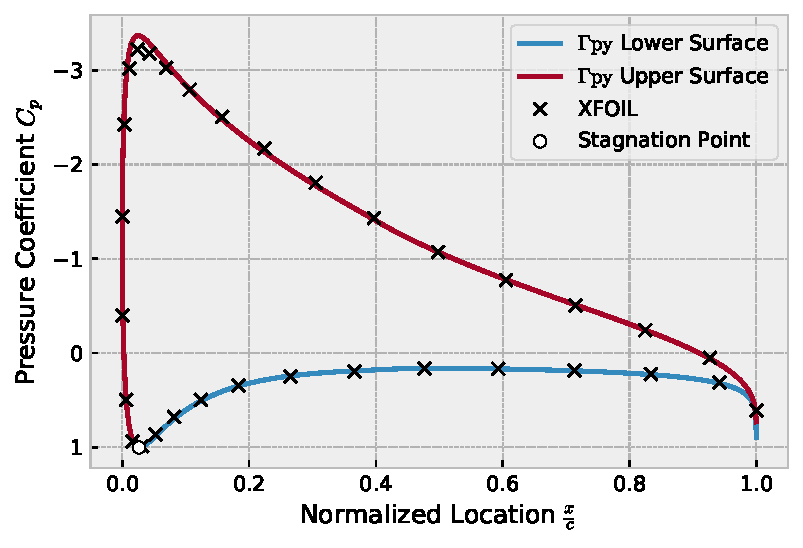
\includegraphics[width=.9\linewidth]{static/thick_verif_naca2422_alpha10.pdf}
      \caption{\centering Pressure distribution NACA2422 at $\alpha = 10^{\circ}$}
      \label{fig:thick_verif2}
    \end{subfigure}
    \caption{\centering Validation of linear vortex method results with \xfoil\cite{xfoil}}
    \label{fig:thick_verif}
\end{figure}


Looking at the resulting estimation for $C_l$, shown in \autoref{tab:cl_thick},
it can be seen that the calculated values for the lift coefficient are slightly
below the values returned by \xfoil for the symmetrical airfoil, and vice versa
for the cambered airfoil tested. For the NACA0015, the relative error $\epsilon$
is zero for $\alpha=0$, and increases with angle of attack. When
$\alpha=10\deg$, the error has risen to $\epsilon=-0.66\%$ (the minus indication
the obtained values are lower than the one returned by \xfoil). The opposite is
true for the NACA2422 results, where the error $\epsilon$ is lowest when
$\alpha$ is high, and increases with decreasing angle of attack. The value of
the error also reaches higher values, namely $\epsilon=+4.58\%$ at
$\alpha=0\deg$.
% These results are also shown as plots in \autoref{fig:cl_thick}

\begin{table}[]
	\centering
	\caption{Estimated values of $C_l$ for a range of angles of attack from \xfoil and NumFoil, as well as the relative error, for NACA0012 and NACA4412.}
	\label{tab:cl_thick}
    \begin{tabularx}{\textwidth}{C  C C C | C C C} %'L' for Left Aligned, 'C' for Centered, 'R' for Right Aligned
    \toprule\
    \hfill & \multicolumn{3}{c}{$C_l$ NACA0015} & \multicolumn{3}{c}{$C_l$ NACA2422} \\ \toprule
    {$\alpha \:[\deg]$} & {$NumFoil$} & {$\xfoil$} & {$\epsilon$} & {$NumFoil$} & {$\xfoil$} & {$\epsilon$} \\ \toprule
    0   & 0        & 0      & 0         & 0.2868 & 0.2742  & +0.0458    \\ \hdashline
    3   & 0.3687   & 0.3708 & -0.0054   & 0.6745 & 0.6645  & +0.0150    \\ \hdashline
    5   & 0.6140   & 0.6175 & -0.0056   & 0.9320 & 0.9238  & +0.0088    \\ \hdashline
    8   & 0.9802   & 0.9861 & -0.0060   & 1.3159 & 1.3105  & +0.0041    \\ \hdashline%\midrule
    10  & 1.2227   & 1.2304 & -0.0062   & 1.5698 & 1.5663  & +0.0022    \\ \hdashline
    13  & 1.5834  & 1.5939 & -0.0066   & 1.9468 & 1.9464  & +0.0002     \\ \bottomrule
    \end{tabularx}
\end{table}

% \begin{figure}[h]
%   \centering
%   \begin{subfigure}{.5\textwidth}
%     \centering
%     \captionsetup{width=.8\linewidth}
%     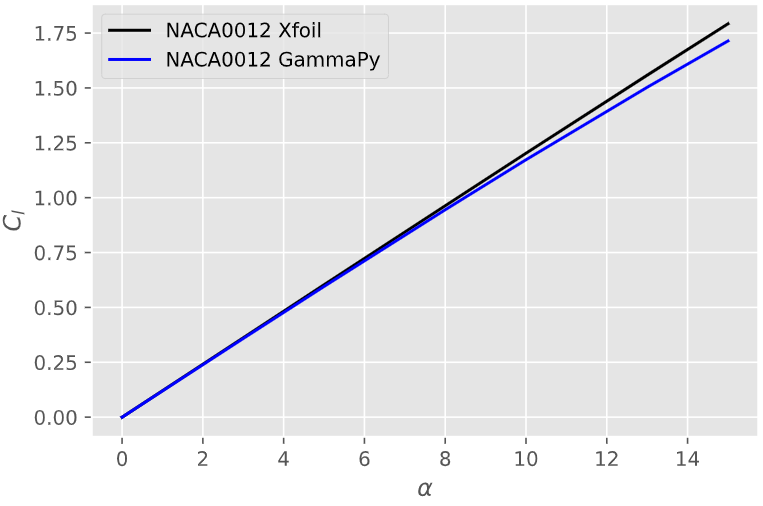
\includegraphics[width=.9\linewidth]{static/naca0012_cl_verif.png}
%     \caption{\centering $C_l - \alpha$ plots for NACA0012}
%     \label{fig:cl_thick_0012}
%   \end{subfigure}\hfill% or \hspace{5mm} or \hspace{0.3\textwidth}
%   \begin{subfigure}{.5\textwidth}
%     \centering
%     \captionsetup{width=.9\linewidth}
%     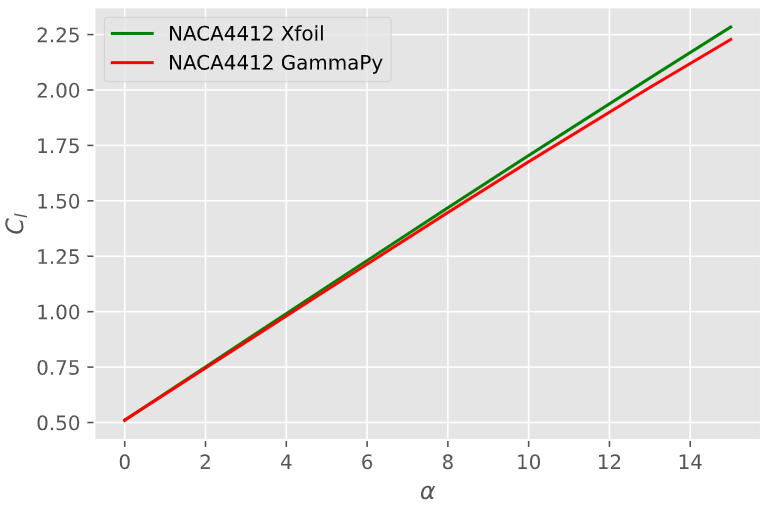
\includegraphics[width=.9\linewidth]{static/naca4412_cl_verif.png}
%     \caption{\centering $C_l - \alpha$ plots for NACA0012}
%     \label{fig:cl_thick_4412}
%   \end{subfigure}
%   \caption{\centering Comparing  $C_l - \alpha$ with results from \xfoil for NACA0012 and NACA4412}
%   \label{fig:cl_thick}
% \end{figure}

% ###########################################################################################
% ###########################################################################################
\chapter{Analysis}
Now that the program is validated, the different aspects of airfoils can be
looked at. First, the effect of camber is discussed in \autoref{sec:camber}.
Next, the change in results due to varying panel thickness is evaluated in
\autoref{sec:thickness}, and, finally, the effect of panel density on the
obtained results is checked in \autoref{sec:panels}.

\section{Effect of Camber}
\label{sec:camber}
To see the effect of varying camber on the results, both the paneled
camberline and paneled surface methods will be used on a set of
airfoils (see \autoref{fig:camber}) where only the camber value is
different. The first one, NACA0015, is a symmetrical airfoil and thus has zero
camber. Subsequent airfoils, NACA2415 and NACA4415 have a respective
maximum camber of 0.2 and 0.4 at $\frac{x}{c}=0.4$. \autoref{fig:camber1}
plot the pressure distributions obtained using the linear vortex method, and
\autoref{fig:camber2} shows the pressure differential plots resulting from the
lumped vortex method.

\begin{figure}[h]
    \centering
    \begin{subfigure}{.5\textwidth}
      \centering
      \captionsetup{width=.8\linewidth}
      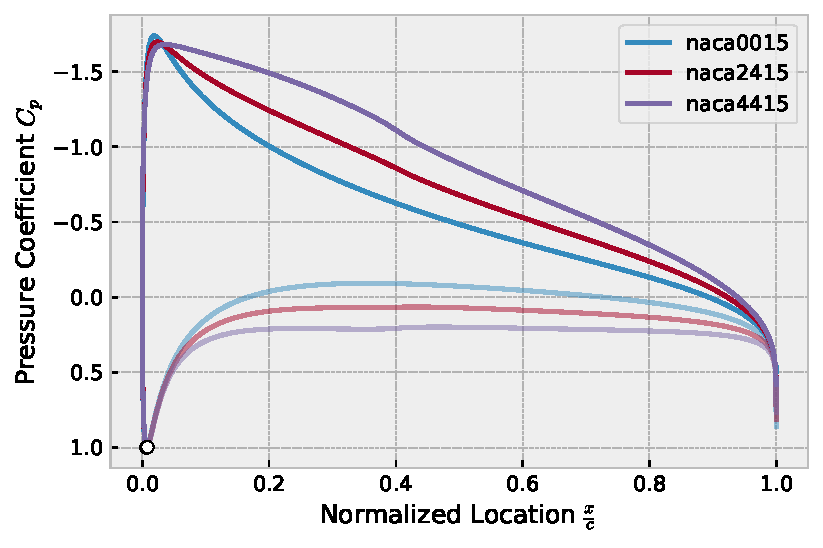
\includegraphics[width=.9\linewidth]{static/thick_camber_a5.pdf}
      \caption{\centering Pressure distributions with varying camber at $\alpha
      = 5^{\circ}$ using the linear vortex method}
      \label{fig:camber1}
    \end{subfigure}\hfill% or \hspace{5mm} or \hspace{0.3\textwidth}
    \begin{subfigure}{.5\textwidth}
      \centering
      \captionsetup{width=.8\linewidth}
      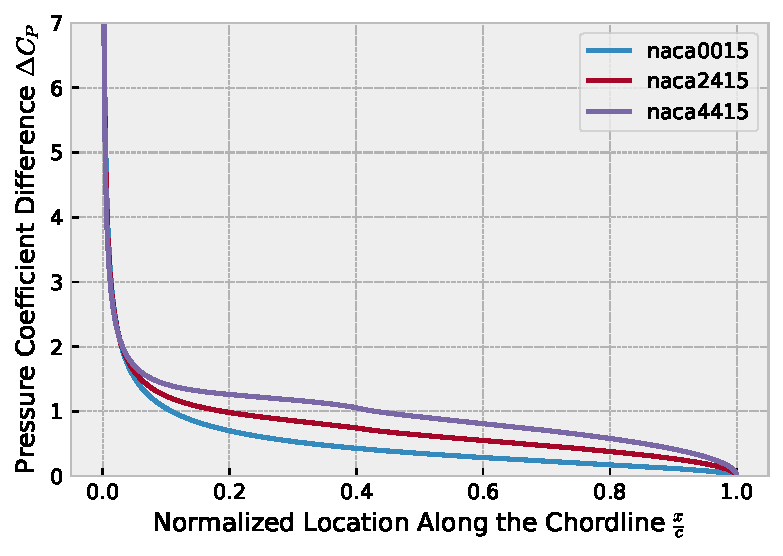
\includegraphics[width=.9\linewidth]{static/thin_camber_a5.pdf}
      \caption{\centering Pressure distributions with varying camber at $\alpha
      = 5^{\circ}$ using the lumped vortex method}
      \label{fig:camber2}
    \end{subfigure}
    \caption{\centering Plots showing the effect of camber on the pressure distribution on airfoils with equal thickness and maximum camber location}
    \label{fig:camber}
\end{figure}

Clearly, a higher camber value leads to higher local values for the (delta) pressure
coefficient. This means the plotted lines representing the $C_p$ of the upper
and lower surfaces lie further apart in \cref{fig:camber1}. This increase in pressure difference in
turn results in a higher value for the lift coefficients.
\medskip

The same is true for the lift polars, as shown in \autoref{fig:cambercl}.
\autoref{fig:cambercl1} shows the changes in lift polar resulting from the
linear vortex model, and \autoref{fig:cambercl2} the same data but now obtained
using lumped vortex model. The plots show that regardless of the method used,
the lift gradient stays constant with increasing camber, but the lift
coefficient values for constant angles of attack increase with camber. Note that
while the airfoil NACA codes in \cref{fig:cambercl2} show a thickness of 0.15,
the lumped vortex model reduces them to zero-thickness plates. Hence why the
symmetrical NACA0015, which is just a flat plate in this model, has a lift
polar which coincides with the theoretical gradient value of $C_{l_\alpha} = 2\pi$.
% Angle of attack clearly has no effect on how much the camber increases
% the lift coefficient, as the lines of different values for $\alpha$ ahave equal
% gradients for every camber value.

% \begin{figure}[h]
%     \centering
%     \begin{subfigure}{.5\textwidth}
%       \centering
%       \captionsetup{width=.8\linewidth}
%       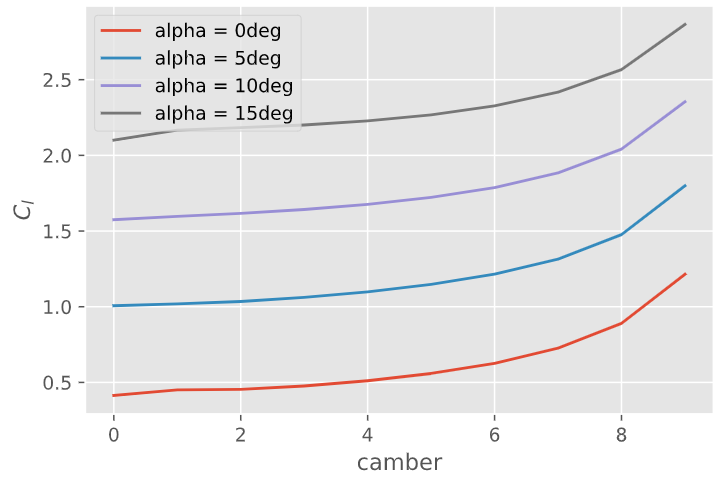
\includegraphics[width=.9\linewidth]{static/cambereffect_thick.png}
%       \caption{\centering Variation of $C_l$ with camber for NACA4X12}
%       \label{fig:cambercl1}
%     \end{subfigure}\hfill% or \hspace{5mm} or \hspace{0.3\textwidth}
%     \begin{subfigure}{.5\textwidth}
%       \centering
%       \captionsetup{width=.9\linewidth}
%       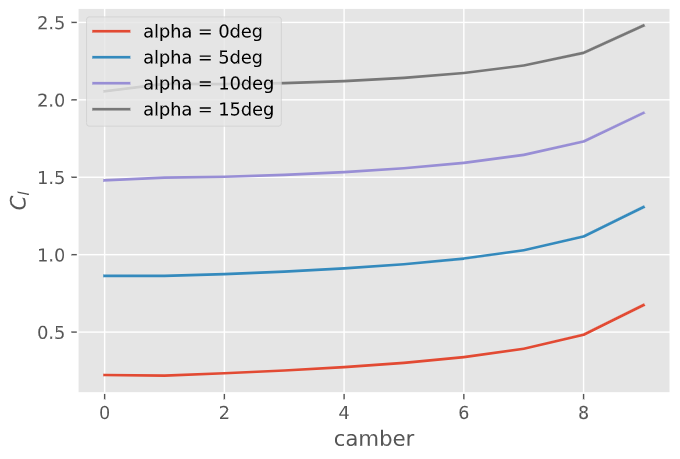
\includegraphics[width=.9\linewidth]{static/cambereffect2_thick.png}
%       \caption{\centering Variation of $C_l$ with camber for NACA2X22}
%       \label{fig:cambercl2}
%     \end{subfigure}
%     \caption{\centering Variation of $C_l$ with increasing camber for different angles of attack. The X in the NACA codes is the camber which is varied.}
%     \label{fig:cambercl}
% \end{figure}
\begin{figure}[h]
  \centering
  \begin{subfigure}{.5\textwidth}
    \centering
    \captionsetup{width=.8\linewidth}
    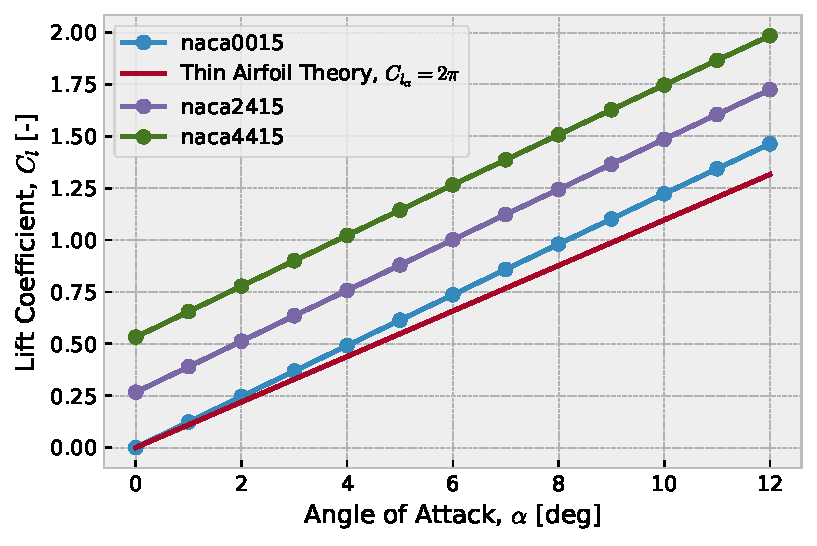
\includegraphics[width=.9\linewidth]{static/thick_camber_cla.pdf}
    \caption{\centering Linear vortex method}
    \label{fig:cambercl1}
  \end{subfigure}\hfill% or \hspace{5mm} or \hspace{0.3\textwidth}
  \begin{subfigure}{.5\textwidth}
    \centering
    \captionsetup{width=.8\linewidth}
    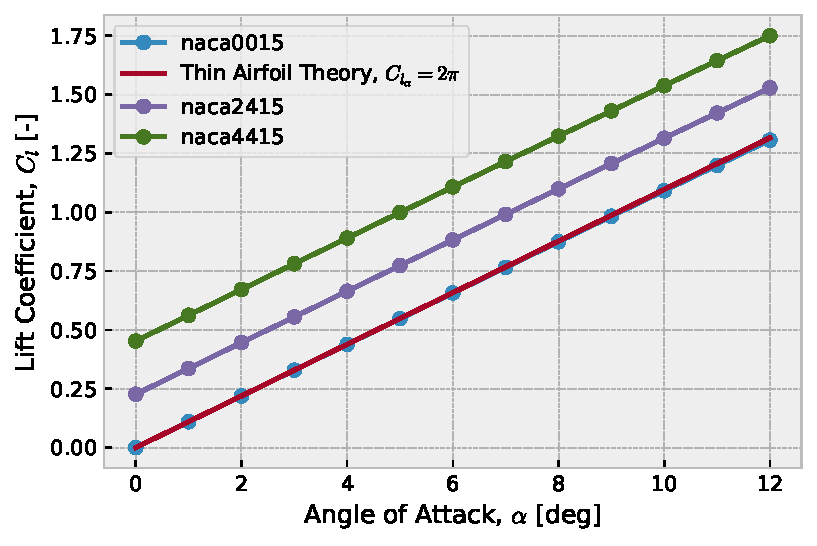
\includegraphics[width=.9\linewidth]{static/thin_camber_cla.pdf}
    \caption{\centering Lumped vortex method}
    \label{fig:cambercl2}
  \end{subfigure}
  \caption{\centering Change of lift polar with increasing camber}
  \label{fig:cambercl}
\end{figure}

% ###########################################################################################
% ###########################################################################################
\section{Effect of Airfoil Thickness}
\label{sec:thickness}
For the lumped vortex method, with a panelled camberline, the thickness will not
have any effect on the results, as can be seen in \cref{fig:thin_tc}. This
method only looks at the camberline, and ignores the airfoil's thickness.
Instead, to evaluate the effect of thickness, the linear vortex method from
\autoref{sec:thick} can be used for this. Pressure distribution plots, obtained
using the linear vortex model, for symmetric airfoil with different thickness
values are shown in \cref{fig:thick_tc}.
The angle of attack is constant for all
cases: $\alpha = 5^{\circ}$. The pressure distributions show that an increase in
thickness reduces the suction peak on the leading edge, while increasing the
pressure deferential over the rest of the airfoil, leading to a net increase in
lift.
\medskip

Comparing the plots for a thin airfoil (\cref{fig:thin_tc} or NACA0001 in
\cref{fig:thick_tc}), it can be seen that the biggest difference is the pressure
at the leading edge. Thin or flat-plate airfoils have a (near) zero-radius
leading edge, cause a very large or even infinite pressure spike and lower
pressure differential across the rest of the airfoil. This pressure spike will
result in very early separation at increased angles of attack. Thicker airfoils
on the other hand have a much lower suction peak on the leading edge. They are
thus capable of achieving much higher angles of attack due to the absence of
this strong adverse pressure gradient.

\begin{figure}[h]
  \centering
  \begin{subfigure}{.5\textwidth}
    \centering
    \captionsetup{width=.8\linewidth}
    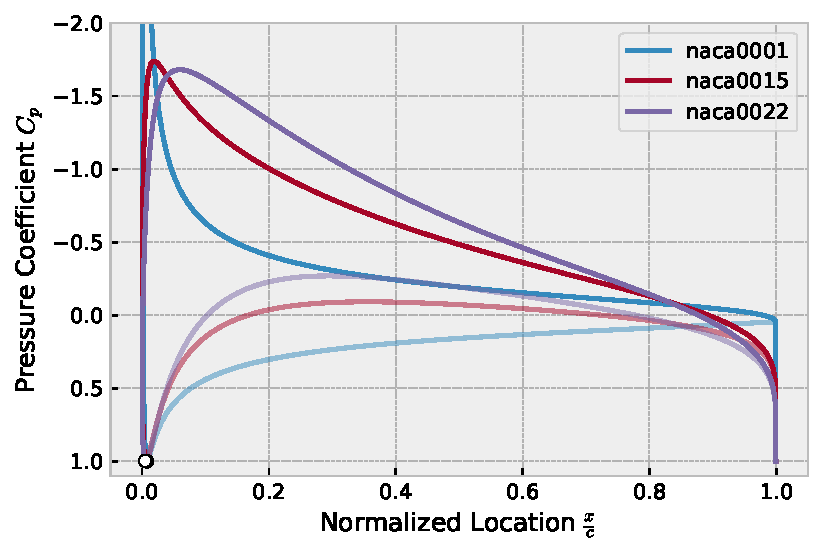
\includegraphics[width=.9\linewidth]{static/thick_tc_a5.pdf}
    \caption{\centering Pressure distributions for varying thickness using the linear vortex method}
    \label{fig:thick_tc}
  \end{subfigure}\hfill% or \hspace{5mm} or \hspace{0.3\textwidth}
  \begin{subfigure}{.5\textwidth}
    \centering
    \captionsetup{width=.8\linewidth}
    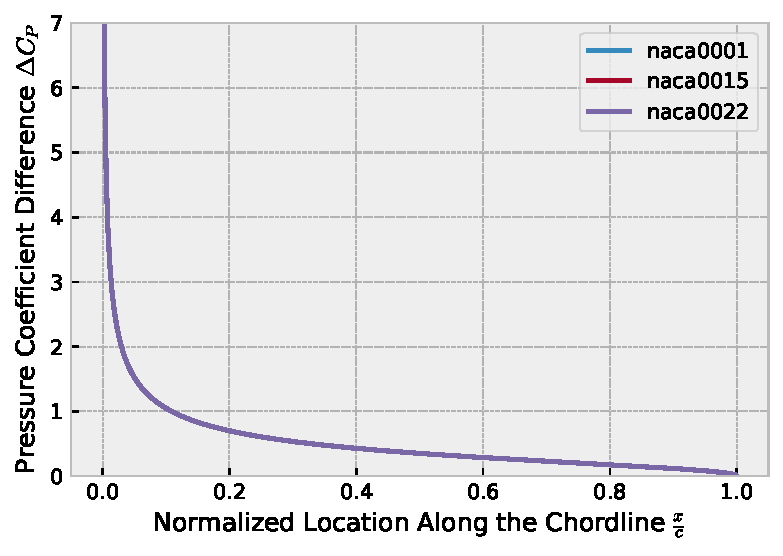
\includegraphics[width=.9\linewidth]{static/thin_tc_a5.pdf}
    \caption{\centering  Pressure distributions for varying thickness using the lumped vortex method}
    \label{fig:thin_tc}
  \end{subfigure}
  \caption{\centering Effect of thickness on the pressure distribution for a symmetric airfoil at $\alpha = 5^{\circ}$.}
  \label{fig:thickcp}
\end{figure}

The changes in lift polar with increasing thickness can be observed in
\autoref{fig:tc_cla}. Once more, as expected the lumped vortex method does not
show any changes with varying thickness, and lift polars coincide with the
theoretical lift polar corresponding to a lift gradient of  $C_{l_\alpha} =
2\pi$.
The lift polars obtained using the linear vortex model show an increase in the
lift gradient (slope of the $C_l-\alpha$ curve) with increasing thickness. Since
the polars go through the origin of the plot, the
exact value of the lift gradient can be determined by, e.g., taking the value of
$C_l$ at $\alpha=\SI{10}{\degree}$ and dividing that value of $C_l$ by the
equivalent of \SI{10}{\degree} in radians. This basically comes down to finding
$C_{l_\alpha}=\frac{\Delta C_l}{\Delta \alpha}$.

\begin{figure}[h]
  \centering
  \begin{subfigure}{.5\textwidth}
    \centering
    \captionsetup{width=.8\linewidth}
    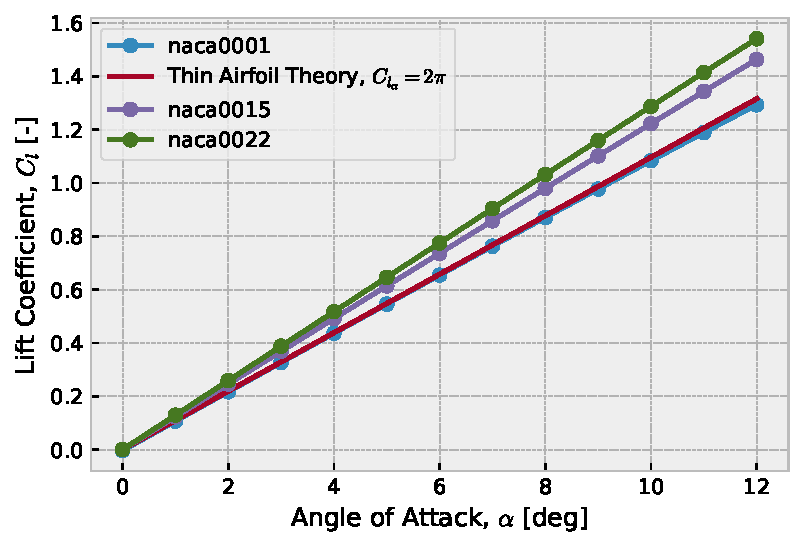
\includegraphics[width=.9\linewidth]{static/thick_tc_cla.pdf}
    \caption{\centering Lift polar for varying thickness using the linear vortex method}
    \label{fig:thick_tc_cla}
  \end{subfigure}\hfill% or \hspace{5mm} or \hspace{0.3\textwidth}
  \begin{subfigure}{.5\textwidth}
    \centering
    \captionsetup{width=.8\linewidth}
    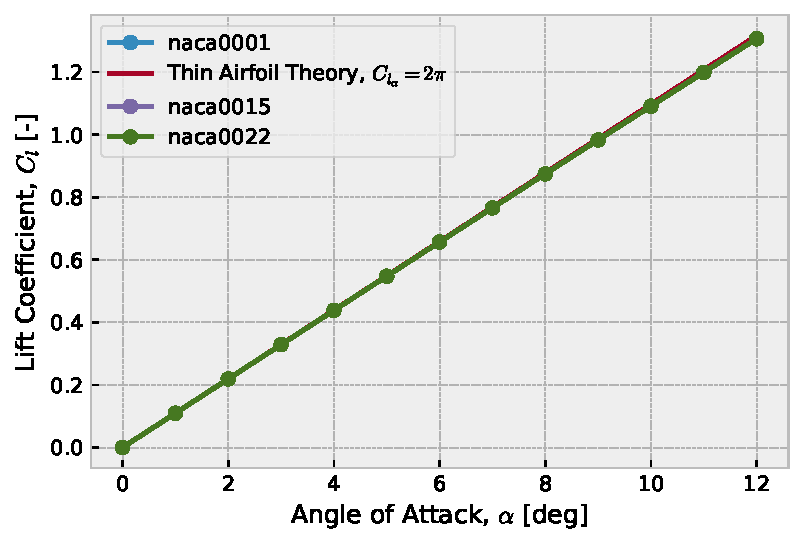
\includegraphics[width=.9\linewidth]{static/thin_tc_cla.pdf}
    \caption{\centering Lift polar for varying thickness using the lumped vortex method}
    \label{fig:thin_tc_cla}
  \end{subfigure}
  \caption{\centering Effect of thickness on the $C_l$ for a symmetric airfoil at different angles of attack.}
  \label{fig:tc_cla}
\end{figure}


% ###########################################################################################
% ###########################################################################################
\section{Effect of Panel Density}
\label{sec:panels}
Varying the panel density of course will also vary the fidelity of the analysis.
\autoref{fig:npanels} shows the effect of increasing the amount of panels on the
resulting pressure distribution. Clearly a larger number of panels leads to more
accurate results. Note that the amount of panels is the total amount for the
linear vortex method, meaning the upper and lower airfoil surface each half of
this amount of panels. To determine the recommended amount of panels, the lift
coefficient is calculated for an increasing amount of panels, until the relative
error is less than $\epsilon < 0.5\%$. The result are shown in
\cref{fig:thick_panels}, where \cref{fig:thick_panels1} does this for the
NACA0015 at $\alpha=\SI{5}{\degree}$, and \cref{fig:thick_panels2} for the
NACA2422 at $\alpha=\SI{10}{\degree}$. With this criterion, the recommended
minimum amount of panels lies around $n_{panels} = \pm 100$, which means at least 50
panels when using the lumped vortex method, but due to the flat-plate
assumption, this method will always have higher error values. For reference, the
default number of panels that \xfoil uses is 160.


\begin{figure}[h]
  \centering
  \begin{subfigure}{.5\textwidth}
    \centering
    \captionsetup{width=.8\linewidth}
    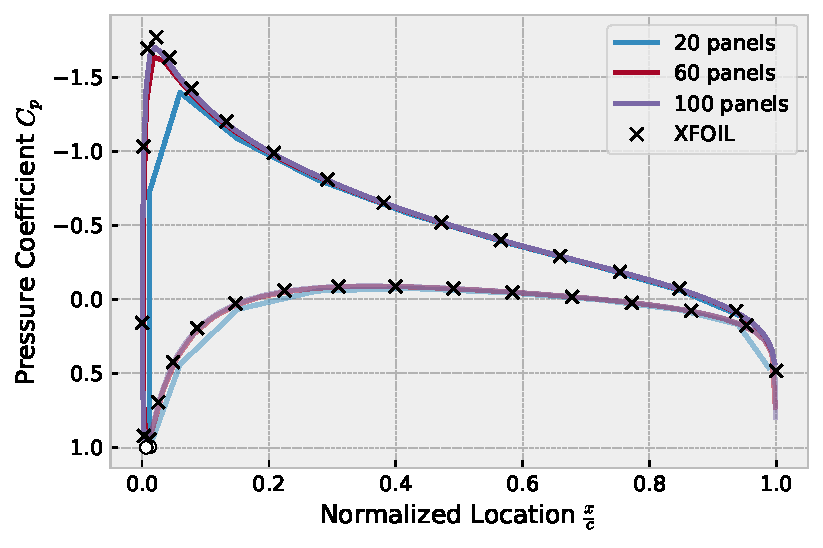
\includegraphics[width=.9\linewidth]{static/thick_panels.pdf}
    \caption{\centering Pressure distributions using the linear vortex model}
    \label{fig:thick_npanels}
  \end{subfigure}\hfill% or \hspace{5mm} or \hspace{0.3\textwidth}
  \begin{subfigure}{.5\textwidth}
    \centering
    \captionsetup{width=.8\linewidth}
    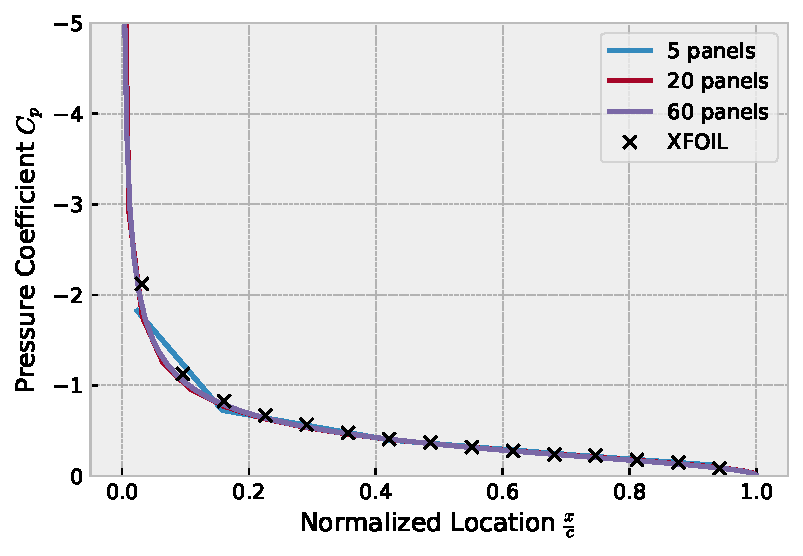
\includegraphics[width=.9\linewidth]{static/thin_panels.pdf}
    \caption{\centering  Pressure differential distributions using the lumped vortex model}
    \label{fig:thin_npanels}
  \end{subfigure}
  \caption{\centering Pressure distributions for the NACA0015 at
  $\alpha=\SI{5}{\degree}$ with varying panel density}
  \label{fig:npanels}
\end{figure}

\begin{figure}[h]
  \centering
  \begin{subfigure}{.5\textwidth}
    \centering
    \captionsetup{width=.8\linewidth}
    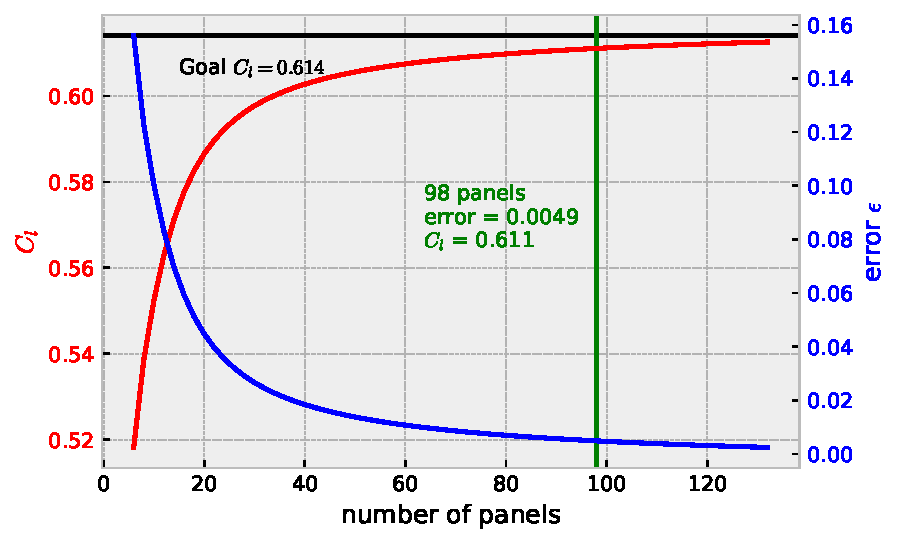
\includegraphics[width=.9\linewidth]{static/thin_conv_naca0015.pdf}
    \caption{\centering Panels required for a NACA0015 at $\alpha = 5^{\circ}$}
    \label{fig:thick_panels1}
  \end{subfigure}%
  \begin{subfigure}{.5\textwidth}
    \centering
    \captionsetup{width=.8\linewidth}
    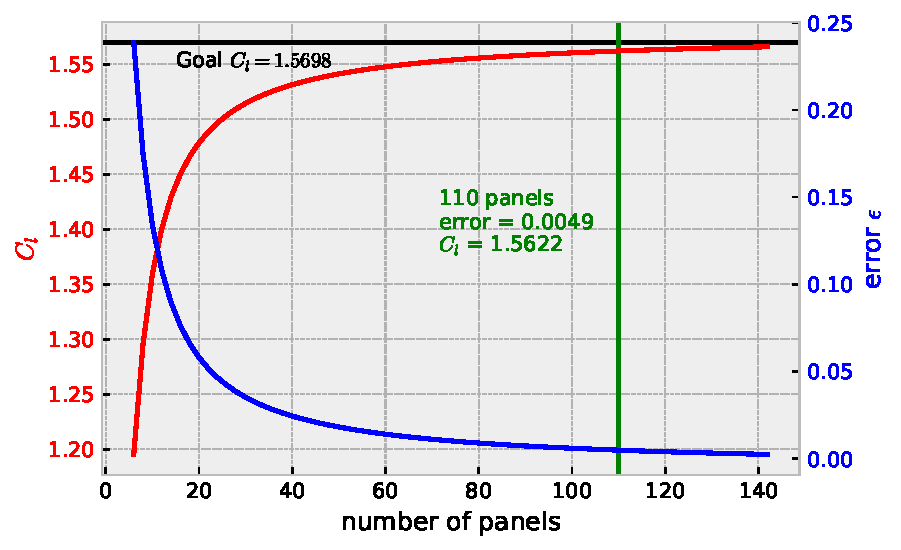
\includegraphics[width=.9\linewidth]{static/thin_conv_naca2422.pdf}
    \caption{\centering Panels required for a NACA2422 at $\alpha = 10^{\circ}$}
    \label{fig:thick_panels2}
  \end{subfigure}
  \caption{\centering Convergence of results with increasing panel density}
  \label{fig:thick_panels}
\end{figure}
